\documentclass[a4paper]{article}

\usepackage[english]{babel}
\usepackage[utf8]{inputenc}
\usepackage{amsmath}
\usepackage{graphicx}
\usepackage[colorinlistoftodos]{todonotes}

\usepackage{theorem}
\usepackage{amssymb}

\usepackage{hyperref}

\newenvironment{proof}{{\bf Proof:  }}{\hfill\rule{2mm}{2mm}}

\newtheorem{fact}{Fact}[section]
\newtheorem{lemma}[fact]{Lemma}
\newtheorem{theorem}[fact]{Theorem}
\newtheorem{definition}[fact]{Definition}
\newtheorem{corollary}[fact]{Corollary}
\newtheorem{proposition}[fact]{Proposition}
\newtheorem{claim}[fact]{Claim}
\newtheorem{exercise}[fact]{Exercise}

\newcommand{\RT}[1]{\marginpar{\footnotesize\color{red}RT: #1}}

\title{Outline for LLG}

\date{\today}

\begin{document}
\maketitle

\section{Introduction}

\begin{itemize}
\item Mean is one of the most important and basic concept in statistics. Motivated by the law of large numbers, sample mean is always considered to be the best estimate of the population mean. As a result, nowadays we take averages almost everywhere, from the fundamental elements in Euclidean space to more general objects, like shapes, documents and graphs.

However, contradict to the general intuition, arithmetic average should not be our first choice all the time. In 1955, Stein's paradox shows the inadmissibility of the sample mean when there are more than three normal distributions. The fact that James-Stein estimator dominates the sample mean makes it less preferable to take the average in that situation. 27 years later, Gutmann proved that this cannot occur when the sample spaces are finite. But even when sample mean is admissible, it doesn't close the door of other estimators to be better in some cases. So in a specific situation, for instance in this paper a collection of graphs is considered, there is always a chance to have a better estimator compared to the sample mean.




\item The mean of a collection of graphs can be defined in various ways. One natural definition is the proportion of the existence of an edge between any pair of vertices. Estimating the mean of a population of graphs based on a sample is becoming more and more important both in statistical inference and in various applications like connectomics, social networks, etc.
\item Element-wise maximum likelihood estimate, which happens to be the sample mean in many situations, is a reasonable estimator if we only consider the independent edge graph model without taking any graph structure into account. However, it does not perform very well especially when we have a few observations, which is likely the case in real world.
\item (Challenges) Generally, we don't have any information about the structure of the graphs. So it is hard to take advantage of the unknown graph structure.
\item One of the most important structures is the community structure in which vertices are clustered into different communities such that vertices of the same community behave similarly. The stochastic blockmodel (SBM) captures such structural property and is widely used in modeling networks.
\item Meanwhile, the latent positions model (LPM), a much more general model compared to SBM, proposes a way to parameterize the graph structure by latent positions associated with each vertex. However, the random dot product graph (RDPG) which is a special case of LPM stays in between and motivates our estimator. In this paper, we analyze our estimator in terms of RDPG specifically.
\item Using the estimates of the latent positions in an RDPG setting based on a truncated eigen-decomposition of the adjacency matrix, we consider a new estimator for the mean of the collection of graphs which captures the low-rank structure. And we prove via both theory and simulations/real data analysis that it is better than element-wise MLE.
\item (Future work) Robust estimation, dimension selection, diagonal augmentation, etc.
\end{itemize}


\section{Models and Estimators}

%\begin{itemize}
%\item The goal is to estimate the mean of a collection of unweighted simple graphs by observing their adjacency matrices with known vertex correspondence.
%\item This work considers the scenario of having $M$ graphs represented as adjacency matrices, each having $N$ vertices with known correspondence. And much more detailed description.
%\end{itemize}

%\subsection{Entry-Wise Least Squares Estimate}
\subsection{Independent Edge Model}
\begin{itemize}
\item Under the independent edge model (IEM), each edge $A_{ij}$ independently follows the Bernoulli distribution with parameter $P_{ij}$.
\end{itemize}

\subsection{Estimator $\bar{A}$}
\begin{itemize}
\item Under the IEM, element-wise mean of the adjacency matrices $\bar{A}$ is the MLE as well as the least squared estimate.
\item $\bar{A}$ is unbiased for IEM and has entry-wise variance $\mathrm{Var}(\bar{A}_{ij}) = P_{ij} (1-P_{ij})/M$. And it is the UMVUE under IEG with no constraints. But, it doesn't exploit any structure. 
\end{itemize}

\subsection{Random Dot Product Graph}
\begin{itemize}
\item Hoff et. al. (2002) proposed a model for random graphs called Latent Positions Graph Model.
\item A specific instance of this model that we will examine is the random dot product graph model (RDPG) in which the link function is the dot product, i.e. the probability of an edge being present between two nodes is the dot product of their latent vectors.
\end{itemize}

\subsection{Estimator $\hat{P}$ Based on Adjacency Spectral Embedding}
\begin{itemize}
\item In order to take advantage of the underlying low rank structure of the RDPG, we use the adjacency spectral embedding (ASE) studied by Sussman et. al. to enforce a low rank approximation on the entry-wise mean matrix $\bar{A}$, which will decrease the variance without losing much in bias if we embed it into the right dimension.
\item There are varies ways dealing with dimension selection. In this paper, we consider Zhu and Ghodsi's elbow selection method and the universal singular value thresholding (USVT) method. Details are discussed in Section \ref{section:dim_select}.
\item Detailed description of the algorithm for our estimator $\hat{P}$.
\end{itemize}

\subsection{Stochastic Block Model as a Random Dot Product Graph}
\begin{itemize}
\item One of the most important structures is the community structure in which vertices are clustered into different communities such that vertices of the same community behave similarly. Such structural property is captured by the SBM, where each vertex is assigned to a block and the probability that an edge exists between two vertices depends only on their respective block memberships.
\item Formally, the SBM is determined by the number of blocks K (generally way less than the number of vertices N), block proportion vector $\rho$, and block probability matrix B.
\item Now if we consider the SBM as a random dot product graph, all vertices in the same block would have identical latent positions.
\end{itemize}


\section{Results}

\subsection{Theoretical Results}
\begin{itemize}
\item To compare the performance between $\hat{P}$ and $\bar{A}$, we examine the relative efficiency (RE), in mean squared error (MSE), among the two defined as: $RE_{ij} = \frac{MSE(\hat{P}_{ij})}{MSE(\bar{A}_{ij})}$.
\item
\begin{theorem}
\label{thm:ARE}
For any $i$ and $j$, conditioning on $X_i = \nu_{\tau_i}$ and $X_j = \nu_{\tau_j}$, we have
\[
	\mathrm{ARE}(\bar{A}_{ij}, \hat{P}_{ij}) = 0.
\]
And for $N$ large enough, conditioning on $X_i = \nu_{\tau_i}$ and $X_j = \nu_{\tau_j}$, we have
\[
	\mathrm{RE}(\bar{A}_{ij}, \hat{P}_{ij}) \approx
    \frac{1/\rho_{\tau_i} + 1/\rho_{\tau_j}}{N}.
\]
\end{theorem}
\item
\begin{lemma}
\label{lm:VarPhat}
In the same setting as above, for any $i, j$, conditioning on $X_i = \nu_{\tau_i}$ and $X_j = \nu_{\tau_j}$, we have
\[
	\lim_{n \to \infty} N \cdot \mathrm{Var}(\hat{P}_{ij}) =
    \frac{1/\rho_{\tau_i} + 1/\rho_{\tau_j}}{M} P_{ij} (1 - P_{ij}).
\]
And for $N$ large enough, conditioning on $X_i = \nu_{\tau_i}$ and $X_j = \nu_{\tau_j}$, we have
\[
	E[(\hat{P}_{ij} - P_{ij})^2] \approx
    \frac{1/\rho_{\tau_i} + 1/\rho_{\tau_j}}{M N} P_{ij}(1-P_{ij}).
\]
\end{lemma}
\end{itemize}

\subsection{Validation with Simulations}
\begin{itemize}
\item We demonstrate the theoretical results in Section 3.1, the relative efficiency of $\hat{P}$, via various Monte Carlo simulation experiments.
\end{itemize}
\subsubsection{Simulation Setting}
\begin{itemize}
\item Here we consider the 2-block SBM parameterized by
\begin{equation*}
B = \begin{bmatrix}
0.42 & 0.2 \\
0.2 & 0.7
\end{bmatrix}
,\qquad \rho = \begin{bmatrix}
0.5 & 0.5
\end{bmatrix}.
\end{equation*}
\item And we embed the graphs into the dimension $d = \mathrm{rank}(B) = 2$.
\end{itemize}
\subsubsection{Simulation Results}
\begin{itemize}
\item Figure \ref{fig:RE} plots the scaled average RE with different $N$ and fixed $M$ of 1000 Monte Carlo replicates. Blue lines denote the simulated scaled RE associated with the edges we are averaging over. Solid line in black represents the theoretical value for scaled RE. From the figure, we see that $N \cdot \mathrm{RE}_{st}(\bar{A}, \hat{P})$ converges to $1/\rho_s + 1/\rho_t$ represented as the black solid line, as suggested in Lemma \ref{thm:ARE}. Notice that this means $\mathrm{RE}_{st}(\bar{A}, \hat{P})$ is decreasing at rate $1/N$.
\item To verify Theorem \ref{thm:ARE} and Lemma \ref{lm:VarPhat} hold with different $\rho$, Figure \ref{fig:RErho} shows the average MSE and average RE with $N = 500$ and $M = 100$ while changing $\rho_1$ from 0.1 to 0.9. 
\item By checking the averaging MSE and RE of the two estimates $\hat{P}$ and $\bar{A}$ over 1000 Monte Carlo replicates, we demonstrate that the theoretical results in Section 3.1.
\end{itemize}

\begin{figure}[!htb]
	\centering
	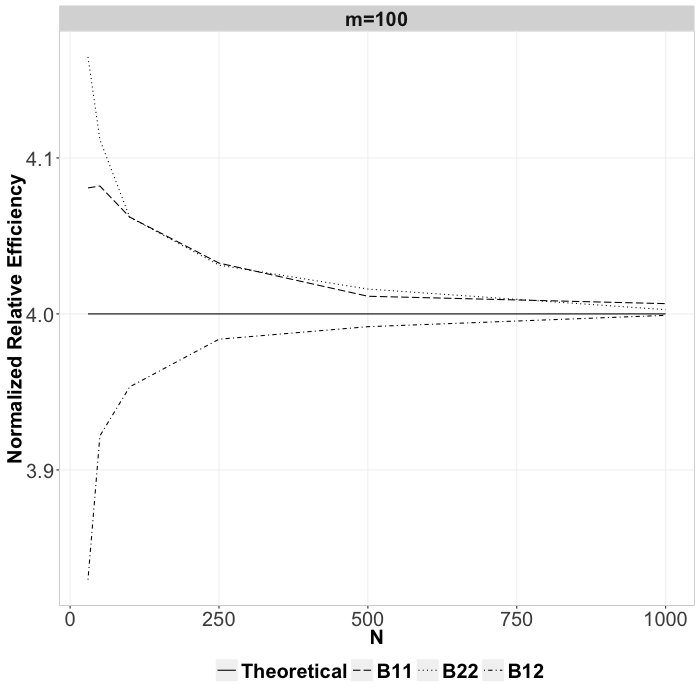
\includegraphics[width=12cm]{RE.png}
	\caption{Scaled average RE with different $N$ and fixed $M$ of 1000 Monte Carlo replicates. Blue lines denote the simulated scaled RE associated with the edges we are averaging over. Dashed lines represent the 95\% confidence interval. Solid line in black represents the theoretical value for scaled RE. Observe that $N \cdot \mathrm{RE}_{st}(\bar{A}, \hat{P})$ converges to $1/\rho_s + 1/\rho_t$ as expected.}
	\label{fig:RE}
\end{figure}

\begin{figure}[!htb]
\centering
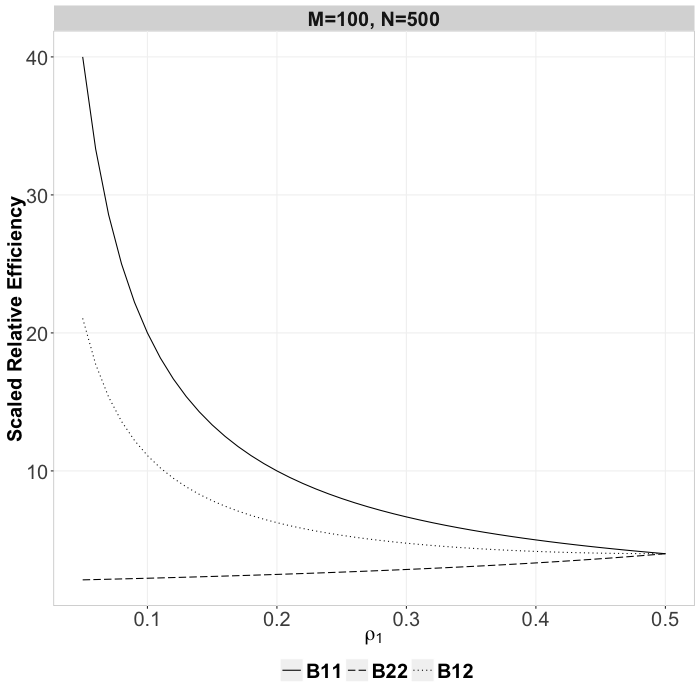
\includegraphics[width=16cm]{Rho.png}
\caption{Simulated results for (a) $\mathrm{MSE}_{st}(\hat{P})$ and (b) $\mathrm{RE}_{st}(\bar{A}, \hat{P})$ with $N = 500$ and $M = 100$ of 1000 Monte Carlo replicates while changing $\rho_1$ from 0.1 to 0.9. Dashed lines represent the 95\% confidence interval. The simulated values for the average MSE and average RE measurements match perfectly with the theoretical values.}
\label{fig:RErho}
\end{figure}

\subsection{CoRR Brain Graphs: Cross-Validation}
\begin{itemize}
\item In practice, the graphs may not perfectly follow an RDPG, or even not IEM. But we are still interested in the mean graph. To demonstrate that the $\hat{P}$ estimate is still valid in such cases, we examine three datasets, JHU, desikan and CPAC200, which are sets of 454 brain connectomes with different number of nodes generated from fMRI scans available at the Consortium for Reliability and Reproducibility (CoRR).
\item To compare $\bar{A}$ and $\hat{P}$ we perform a cross-validation study to examine the impact of the number of available graphs $M$.
\item Figure \ref{fig:JHU}, Figure \ref{fig:desikan} and Figure \ref{fig:CPAC200} demonstrate that our algorithm gives a better estimate $\hat{P}$ according to all three datasets. 
\item When $M$ is small, $\bar{A}$ has large variance which leads to large MSE. Meanwhile, $\hat{P}$ reduces the variance by taking advantages of the graph structure and outperforms $\bar{A}$ dramatically.
\item Moreover, Zhu and Ghodsi's algorithm and USVT algorithm both do a good job for selecting the dimension to embed.
\item Simulation with $P$ being the mean graph of the real data shows that $\hat{P}$ still does a good job when the low rank assumption is violated.
\end{itemize}

\begin{figure}[!htb]
\centering
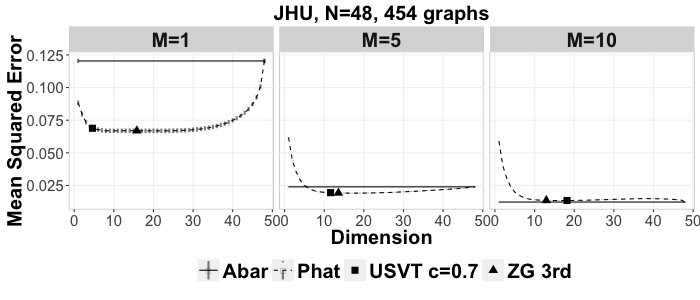
\includegraphics[width=14cm]{JHU.png}
\caption{Comparison of MSE between $\bar{A}$ (red) and $\hat{P}$ (blue) for JHU dataset while embedding the graphs into different dimensions with different size $M$ of the subsamples. The dimension chosen by the 3rd elbow of Zhu and Ghodsi is denoted in purple, and chosen by USVT with threshold equals 0.7 is denoted in green. Dashed lines represent the 95\% confidence interval. When $M$ is small, $\hat{P}$ outperforms $\bar{A}$ with a flexible range of the embedding dimension including what Zhu and Ghodsi selects.}
\label{fig:JHU}
\end{figure}

\begin{figure}[!htb]
\centering
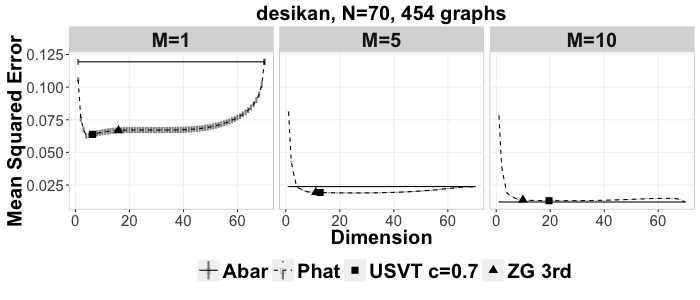
\includegraphics[width=14cm]{desikan.png}
\caption{Comparison of MSE between $\bar{A}$ (red) and $\hat{P}$ (blue) for desikan dataset while embedding the graphs into different dimensions with different size $M$ of the subsamples. The dimension chosen by the 3rd elbow of Zhu and Ghodsi is denoted in purple, and chosen by USVT with threshold equals 0.7 is denoted in green.  Dashed lines represent the 95\% confidence interval.  When $M$ is small, $\hat{P}$ outperforms $\bar{A}$ with a flexible range of the embedding dimension including what Zhu and Ghodsi selects.}
\label{fig:desikan}
\end{figure}

\begin{figure}[!htb]
\centering
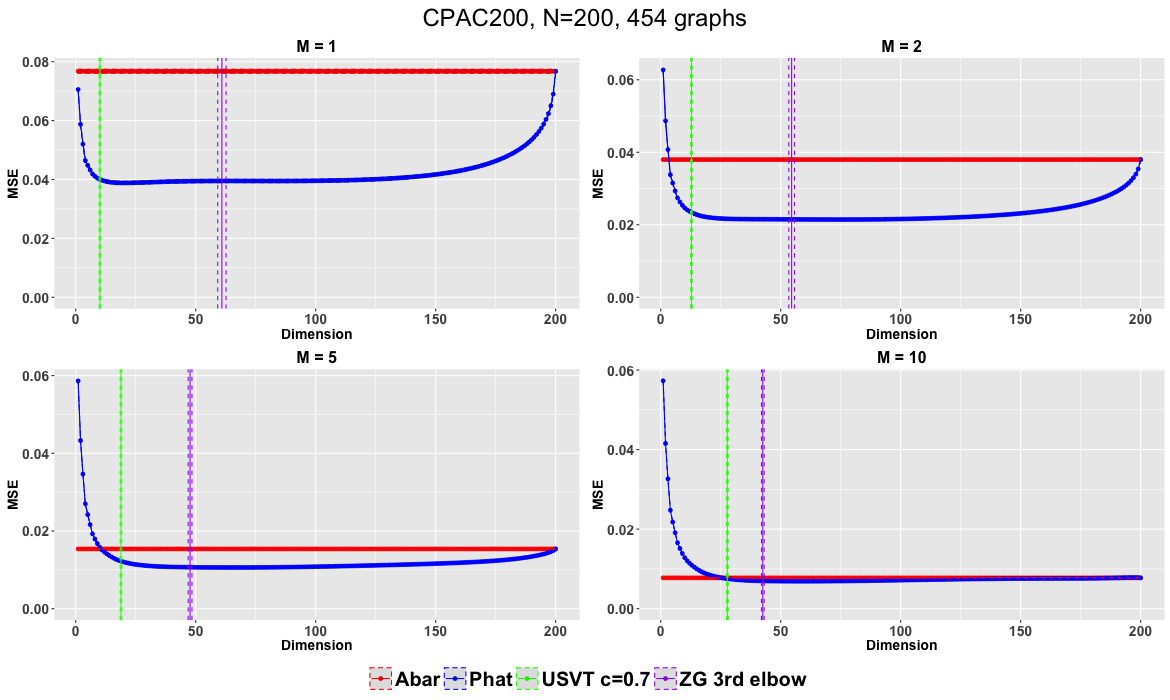
\includegraphics[width=14cm]{CPAC200.png}
\caption{Comparison of MSE between $\bar{A}$ (red) and $\hat{P}$ (blue) for CPAC200 dataset while embedding the graphs into different dimensions with different size $M$ of the subsamples. The dimension chosen by the 3rd elbow of Zhu and Ghodsi is denoted in purple, and chosen by USVT with threshold equals 0.7 is denoted in green.  Dashed lines represent the 95\% confidence interval.  When $M$ is small, $\hat{P}$ outperforms $\bar{A}$ with a flexible range of the embedding dimension including what Zhu and Ghodsi selects.}
\label{fig:CPAC200}
\end{figure}



\section{Discussion}

\subsection{Summary}
\begin{itemize}
\item In this paper, we propose a better way to estimate the mean of a collection of graphs by taking advantage of the low rank structure of the graphs.
\end{itemize}

\subsection{Future Work}
\begin{itemize}
\item Generally the observations we have are always contaminated in practice. In this case, improved robust estimator based on the low rank structure of the graphs is preferred.
\item Estimating the rank of the graph structure accurately will certainly help improve the results.
\item In this paper, we are using Scheinerman's method with 1 iteration for diagonal augmentation.
\end{itemize}






\section{Methods}

\subsection{Choosing Dimension}
\label{section:dim_select}
\begin{itemize}
\item Often in dimensionality reduction techniques, the choice for dimension, d, relies on visually analyzing a plot of the ordered eigenvalues, looking for a ``gap'' or ``elbow'' in the scree-plot.
\item USVT is a simple estimation procedure that works for any matrix that has ``a little bit of structure''.
\end{itemize}

\subsection{Graph Diagonal Augmentation}
\begin{itemize}
\item The graphs examined in this work are hollow, in that there are no self-loops and thus the diagonal entries of the adjacency matrix are 0. This leads to a bias in the calculation of the eigenvectors.
\item We minimize this bias by using an iterative method developed by Scheinerman and Tucker.
\end{itemize}

\subsection{Source Code}

\subsection{Dataset Description}
\begin{itemize}
\item Detailed description of the data we are using.
\end{itemize}

\subsection{Outline for the Proof of the Theorems}







\end{document}